\section{Design Viewpoints}

\subsection{Use Cases}
\label{use-cases}

Een gebruiker kan het systeem anoniem of ingelogd gebruiken. De verschillende functionaliteiten die door deze gebruikt kunnen worden, worden beschreven door verschillende use cases en in het use case diagram samengevat.

\begin{longtable}{lp{10cm}}
Naam           & Account aanmaken.\\
Samenvatting   & De gebruiker maakt een nieuw account aan.\\
Actoren        & Anonieme gebruiker.\\
Aannamen       & \\
Beschrijving   & De anonieme gebruiker vult zijn gegevens in (e-mail, paswoord, voornaam, achternaam, hiërarchische affiliatie en onderzoeksdomein).
Het systeem kijkt na of er al een account met het ingegeven e-mailadres bestaat. Als het account al bestaat, treedt er een uitzondering op.
Daarna kijkt het systeem na of er personen bestaan met de ingegeven naam en voornaam 
(dit is mogelijk indien een vorige gebruiker de naam en voornaam van een persoon die nog geen account heeft, in het systeem heeft ingegeven als co-auteur van zijn paper). 
In dit geval moet de gebruiker zichzelf kiezen uit de gevonden lijst (als hij er tussen zit).
Uiteindelijk maakt het systeem een nieuw account aan.\\
Uitzonderingen & 
\begin{itemize}
\item [bestaand e-mailadres] Het systeem meldt aan dat het e-mailadres al in gebruik is. De gebruiker wordt gevraagd om een ander e-mailadres in te vullen.
\end{itemize}\\
Resultaat      & De gebruiker heeft een account.\\
\end{longtable}

\begin{longtable}{lp{10cm}}
Naam           & Inloggen.\\
Samenvatting   & De gebruiker logt zich in.\\
Actoren        & Anonieme gebruiker.\\
Aannamen       & \\
Beschrijving   & De anonieme gebruiker vult zijn paswoord en e-mailadres in. Het systeem gaat kijken of er al een account met het ingegeven e-mailadres bestaat.
Als dit niet het geval is, treedt er een uitzondering op. Het systeem gaat daarna nakijken of het paswoord van het gevonden account correct is. Zo niet treedt er een uitzondering op.
Uiteindelijk wordt de anonieme gebruiker ingelogd.\\
Uitzonderingen & 
\begin{itemize}
\item [verkeerd e-mail] Het systeem vermeldt dat er geen account met het ingegeven e-mailadres bestaat. De gebruiker wordt gevraagd om zijn e-mailadres opnieuw in te vullen.
\item [verkeerd paswoord] Het systeem vermeldt dat het paswoord voor het gevonden account verkeerd is. De gebruiker wordt gevraagd om zijn paswoord opnieuw in te vullen.
\end{itemize}\\
Resultaat      & De gebruiker is ingelogd.\\
\end{longtable}

\begin{longtable}{lp{10cm}}
Naam           & Publicatie uploaden.\\
Samenvatting   & De gebruiker zet zijn publicatie online.\\
Actoren        & Ingelogde gebruiker.\\
Aannamen       & \\
Beschrijving   & De gebruiker wordt gevraagd om ofwel een pdf bestand, ofwel een bibtex bestand te uploaden. De publicatie-velden worden door het systeem ingevuld indien mogelijk. De gebruiker kan deze zelf nog aanpassen of aanvullen.
Als de gebruiker geen file heeft geüpload, wordt hij gevraagd om manueel alle velden in te vullen. Daarna wordt de publicatie door het systeem toegevoegd.
Als niet alle velden ingevuld zijn treedt er een uitzondering op. Het systeem voegt de publicatie toe aan de gebruikers eigen publicatielijst.\\
Uitzonderingen & 
\begin{itemize}
\item [lege velden] Het systeem toont de niet-ingevulde velden aan, en vraagt de gebruiker om die in te vullen.
\end{itemize}\\
Resultaat      & De gebruiker heeft zijn publicatie geüpload en deze staat in zijn publicatielijst.\\
\end{longtable}

\begin{longtable}{lp{10cm}}
Naam           & Publicaties opzoeken.\\
Samenvatting   & De gebruiker zoekt publicaties op volgens bepaalde criteria.\\
Actoren        & Gebruiker.\\
Aannamen       & \\
Beschrijving   & De gebruiker wordt gevraagd om keywords, disciplines en/of auteurs in te vullen in het zoeksysteem. Het systeem geeft dan de meest relevante publicaties terug.\\
Uitzonderingen & \\
Resultaat      & De meest relevante publicaties worden aan de gebruiker getoond.\\
\end{longtable}


\begin{longtable}{lp{10cm}}
Naam           & Publicatie toevoegen aan gebruiker zijn bibliotheek.\\
Samenvatting   & De gebruiker moet een publicatie die hij gevonden heeft met het systeem kunnen toevoegen aan zijn eigen bibliotheek.\\
Actoren        & Ingelogde gebruiker.\\
Aannamen       & \\
Beschrijving   & De gebruiker zoekt naar publicaties (zie de \textit{use case} "Publicaties opzoeken"). De gebruiker klikt op een gevonden publicatie. Een ingelogde gebruiker krijgt een knop te zien om de publicatie toe te voegen aan zijn bibliotheek. De gebruiker klikt hier op. Hierna verschijnt een kopie van de betreffende publicatie in de bibliotheek van de gebruiker.\\
Uitzonderingen & \\
Resultaat      & De gekozen publicatie bevindt zich in de bibliotheek van de gebruiker.\\
\end{longtable}

%use case template
%\begin{longtable}{lp{10cm}}
%Naam           & \\
%Samenvatting   & \\
%Actoren        & \\
%Aannamen       & \\
%Beschrijving   & \\
%Uitzonderingen & \\
%Resultaat      & \\
%\end{longtable}

\begin{figure}[p]
    \centering
    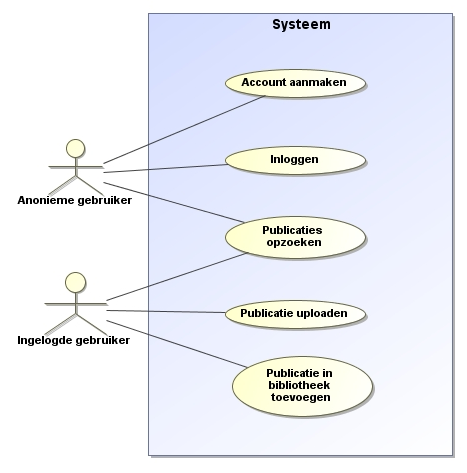
\includegraphics[width=0.8\textwidth]{use-case-diagram}
    \caption{Use Case Diagram}
    \label{fig:use-case-diagram}
\end{figure}